
\chapter{Introduction and Background}

\section{Catalytic Ammonia Synthesis and Its Global Significance}
Catalysis is fundamental to the modern chemical industry. It enables the efficient transformation of raw materials, often derived from fossil resources, into fuels, fertilizers, and commodity chemicals by lowering reaction energy barriers and improving selectivity. The Haber–Bosch synthesis of ammonia is a prime example of how catalysis underpins essential societal functions \cite{Nrskov2016SustainableProduction, Comer2019ProspectsFertilizers, Schloegl2003CatalyticStory}. Developed in the early 20th century, the Haber–Bosch process revolutionized fertilizer production by enabling the conversion of inert atmospheric nitrogen (N$_2$) into reactive ammonia (NH$_3$), producing more than 200 million tonnes annually \cite{MitchellCrow2023AAmmonia, Iriawan_2021}. With a thermochemical efficiency of up to 70\% \cite{Schiffer2017ElectrificationIndustry}, it remains one of the most impactful technologies in industrial chemistry.

The availability of synthetic ammonia-based fertilizers has profoundly shaped global agriculture, sustaining crop yields and enabling large-scale food production \cite{Pinker2018EnlightenmentProgress, Smil1999DetonatorExplosion, Smil2004EnrichingProduction}. As nitrogen depletes from the soil with each harvest, continuous replenishment is essential for maintaining agricultural productivity \cite{Qing2020RecentAmmonia}. By converting atmospheric nitrogen into bioavailable forms, the Haber–Bosch process has enabled sustained agricultural productivity at a global scale. Since 1950, the world population has nearly tripled \cite{UnitedNations2024WorldResults}, a demographic shift made possible in part by the industrial ammonia production. According to Smil, approximately 40\% of global dietary protein in the mid-1990s was attributed to fertilizers produced via this process \cite{Smil2004EnrichingProduction, Gao2023GreenhouseInterventions}.

\section{Limitations of Conventional Ammonia Synthesis}

\subsection{Energy and Emissions from the Haber–Bosch Process}
Although the process has been optimized for energy efficiency over the decades, reducing its carbon footprint remains a significant challenge \cite{Smith2020CurrentLandscape}. The Haber–Bosch method is energy-intensive and carbon-emitting, operating at 650–750 K and 50–200 bar \cite{Comer2019ProspectsFertilizers, Haber1905UberElementen, Tamaru1991CatalyticSynthesis, King1990TheCatalysis, Nielsen1981AmmoniaResearch, Ertl1997HandbookCatalysis, Schloegl2003CatalyticStory, Iriawan_2021, Fernandez2020EditorsParity, Fernandez2020OpportunitiesElectrosynthesis}. The process consumes nearly 1-2\% of global energy \cite{Capdevila-Cortada2019ElectrifyingHaberBosch, Soloveichik2019ElectrochemicalProcess, Kyriakou2020AnProcess}, mainly due to the high kinetic barrier associated with cleaving the $\mathrm{N \equiv N}$ triple bond \cite{vanderHam2014ChallengesTransfer}. Furthermore, the hydrogen feedstock is typically derived from methane steam reforming, contributing approximately 340 million tonnes of CO$_2$ equivalent annually \cite{Abbas2010HydrogenReview}. As a result, the Haber–Bosch process remains one of the largest point sources of industrial greenhouse gas emissions worldwide \cite{Nrskov2016SustainableProduction, Schiffer2017ElectrificationIndustry}.

\subsection{Air Separation and the Need for Selective Catalysis}
In addition to hydrogen, the process uses pure nitrogen feedstocks, which is obtained from energy-intensive air separation units \cite{liu2021prospects}. This requirement further limits the feasibility of decentralized ammonia production. Conducting nitrogen catalysis directly in air is problematic: oxygen dilutes the nitrogen concentration, introduces mass transfer limitations, and competes for  charge carriers in photo- or electrocatalytic systems. This competition not only lowers nitrogen conversion efficiency but also leads to the formation of reactive oxygen species that oxidize the ammonia product, decreasing the product yield \cite{Ye2017Ni2PLight, Huang2020TowardLigands, comer2018role, Smith2020CurrentLandscape}. On some active catalysts, even oxygen and hydroxyl groups from trace water vapor can adsorb and oxidize active surfaces \cite{Rohr2019ACatalysts}. Furthermore, the simultaneous presence of ammonia, hydrogen, and oxygen poses a significant safety risk due to the potential for explosive mixtures \cite{Silverman1938LeAmmonia}. These challenges underscore the importance of developing selective catalysts that can fix nitrogen directly from air, without prior gas purification, especially in decentralized photocatalytic or electrochemical applications.


\subsection{Inequities of Centralized Ammonia Production}
Beyond energy and emissions, the centralized nature of ammonia production introduces significant logistical, environmental, and social challenges. Economies of scale have led to the development of fewer than 100 large-scale ammonia plants worldwide, each with an average capacity of 2200 tonnes per day \cite{McArthur2017FertilizingDevelopment, Bartels2008AEconomy}. These facilities, typically located in economically advantaged regions, can reduce production costs to 300–400 USD per tonne of NH$_3$ \cite{liu2021prospects}. However, ammonia-based fertilizers are often consumed in decentralized and economically disadvantaged regions \cite{Comer2019ProspectsFertilizers}, creating a mismatch between production and need. To minimize transportation costs \cite{BonillaCedrez2020SpatialAfrica, Srivastava2023ProspectsFertilizers}, the industry has shifted toward manufacturing solid and highly concentrated fertilizer products. While this strategy improves logistics, it has introduced new challenges related to safety, equity, and environmental sustainability.

In remote regions such as sub-Saharan Africa, limited infrastructure and high fertilizer prices restrict access for smallholder and resource-poor farmers, contributing to significantly lower fertilizer usage and reduced crop yields compared to other regions \cite{Gilbert2012AfricanPoor, Mueller2012ClosingManagement, vanderVelde2014AfricanConsumption, Erisman2008HowWorld}. In contrast, developed areas often face the opposite problem: the excessive application of fertilizers has led to nitrate leaching, eutrophication, and increased emissions of nitrous oxide—a potent greenhouse gas \cite{ West2002AStates, Diaz2008SpreadingEcosystems, Stevens2019NitrogenEnvironment}. These disparities have intensified interest in decentralized ammonia synthesis approaches that could democratize access to fertilizers \cite{Tonelli2024Cost-competitiveSecurity, DAngelo2023EnvironmentalEnergy, Martin2019ElectrocatalyticLeaf}. Achieving this goal will require the development of modular, small-scale reactors that can operate under mild conditions and be powered by renewable energy.


\section{Alternative Nitrogen Fixation Technologies}
In response to the growing urgency of decarbonizing, researchers have devoted considerable efforts to innovating ways to reduce the energy consumption of the Haber–Bosch process and its related CO$_2$ emissions. For example, by integrating carbon capture technologies, replacing fossil-derived hydrogen with green hydrogen from water electrolysis, and developing catalysts that enable milder operating conditions \cite{2023GreenSynthesis, Torrente-Murciano2023ProcessProduction, Ye2023ProspectsSynthesis, Gabrielli2023Net-zeroResources, Rosa2023EnergyEmissions, Gabrielli2020TheIndustry, Aika1972ActivationMetal, Sato2017ASynthesis, Kitano2018Self-organizedSynthesis}. However, such improvements are only applied to centralized facilities and require a high capital investment. Therefore, increasing catalysis research efforts have shifted toward developing decentralized, modular alternatives that can operate under ambient or electrochemical conditions. Most investigations of these next-generation systems focus on four main strategies: electrocatalysis \cite{Foster2018CatalystsAmmonia, Wang2018AmbientOverpotential, Westhead2021IsElectroreduction, Bagger2021RoleElectrodes}, plasma-based catalysis \cite{Gorbanev2024PlasmaIt, Hong2017PlasmaProgress, Rouwenhorst2021Plasma-catalyticPlasma, Sun2021AProduction}, mechanocatalysis \cite{Reichle2024MechanocatalyticPathway, DeWitt2023StructuralSynthesis, Tricker2020MechanocatalyticMicroenvironments}, and photocatalysis \cite{comer2018role, Huang2023FormationIllumination, Tian2023ScreeningAir, Zhang2019PhotocatalyticFuture}.

\subsection{Electrocatalysis}
Electrochemical nitrogen reduction offers a decentralized and sustainable alternative to the Haber–Bosch process by enabling ammonia synthesis under ambient conditions using renewable electricity and water as the hydrogen source \cite{Greenlee2018TheDinitrogen, Foster2018CatalystsAmmonia}. It can be implemented in small-scale systems powered by solar or wind. A key challenge in this method is to develop active and selective catalysts such that N$_2$ is adsorbed on active sites selectively, competing against the hydrogen evolution reaction (HER) \cite{Singh_2017}. Noble metals (e.g. Au, Pd, Ru) and transition metals (e.g. Mo) have shown promising performance \cite{Wang2018AmbientOverpotential, Bao2017ElectrochemicalCycle, Cheng2018MolybdenumConditions}, but current materials generally suffer from low activity, poor selectivity, and Faradaic efficiencies below 10\% \cite{R.Singh2016ElectrochemicalChallenge, Giddey2013ReviewMaterials, Guo2018RationalConditions, Cui2018AConditions, Kyriakou2017ProgressAmmonia}. Emerging strategies such as gas diffusion electrodes \cite{Fu2023Continuous-flowOxidation}, lithium- and calcium-mediated pathways \cite{McEnaney2017AmmoniaPressure, Li2021EnhancementOxygen, Suryanto2021NitrogenShuttle, Cai2021Lithium-mediatedPerformance, Fu2024Calcium-mediatedSynthesis},  and solid-electrolyte interphases \cite{Li2022ElectrosynthesisInterphase} aim to suppress HER and improve N$_2$ diffusivity near catalyst surfaces. Nonetheless, issues such as catalyst corrosion, lower reaction rates, and false positives in product detection still remain. Additionally, nearly all improved technologies to date rely on purified N$_2$ feedstocks from energy-intensive upstream air separation. Addressing these limitations will require continued efforts in catalyst and reactor design.


\subsection{Plasma-Activated Processes}

Plasma-activated nitrogen fixation offers a decentralized and potentially fossil-free route to ammonia synthesis by using electrical energy to generate reactive species that activate N$_2$ under ambient conditions \cite{Mehta2019CatalysisReview, Bogaerts2018PlasmaStorage, Zhao2023SustainableInteractions, Gorbanev2024PlasmaIt, Sharma2021PlasmaWater, Gao2023Plasma-ActivatedAeroponics}. In non-thermal plasmas, excited electrons induce excitation, ionization, and dissociation of N$_2$ without significantly heating the bulk gas, allowing nitrogen fixation at atmospheric pressure. This approach can be powered by renewable electricity and coupled with H$_2$ from water electrolysis or, in some cases, water vapor alone \cite{Pfromm2017TowardsAmmonia}. Plasma catalysis may also overcome the linear scaling relationship between N adsorption strength and activation energy, expanding the range of effective catalysts beyond those used in thermocatalysis \cite{Chen2018BeyondTransformations, Mehta2018OvercomingCatalysis, Wang2019Plasma-EnhancedMechanism, Peng2019SustainableCatalysis, Mehta2019CatalysisReview, Patil2015Plasma19002014, Carreon2019PlasmaDirections, Rouwenhorst2020Plasma-drivenElectricity, Rouwenhorst2021Plasma-catalyticPlasma}. However, the unit energy efficiency of plasma ammonia synthesis usually range from from 0.3-3g NH$_3$/kWh \cite{Bai2003PlasmaPressure, Bai2008SynthesisCondition}, while Haber–Bosch can reach 127g NH$_3$/kWh \cite{Patil2015Plasma19002014, Chen2021ReviewTechnology}. 
  


\subsection{Mechanocatalysis}
Mechanochemistry offers a novel approach to distributed ammonia production, utilizing mechanical energy to drive chemical reactions in the solid state. Although mechanochemistry has been widely applied in fields such as materials synthesis \cite{Uzarevic2015Real-TimeChemists, Weidenthaler2009ComplexStorage} and heterogeneous catalysis \cite{Bilke2019MethanePathway, Bolm2019MechanochemistryReactants}, its application to nitrogen fixation is relatively recent. In these approaches, the mechanical energy derived from ball grinding can create thermal hot spots, reactive interfaces, and active defect sites \cite{Tricker2020MechanocatalyticMicroenvironments, Suryanarayana2001MechanicalMilling,Immohr2013AnMilling,Schreyer2017OscillatoryCatalysts,Takacs2013TheMechanochemistry, Yu2025EvaluatingOxide}. This solid-state approach only requires localized energy input, eliminating the need for high temperatures or pressures, and thus enabling nitrogen fixation under nominally ambient conditions. Transition metal catalysts such as iron, ruthenium and titanium have shown mechanocatalytic activity, with ammonia formation demonstrated under continuous N$_2$ gas flow during mechanical activation \cite{Heinicke1961DieKatalysators, Peter1974ZurWasser, Reichle2024MechanocatalyticPathway, Reichle2021MechanocatalyticPressure, Tricker2020MechanocatalyticMicroenvironments}. One of the main advantages of this approach lies in its simplicity: it does not require complex catalyst synthesis, and it has demonstrated ammonia yields orders of magnitude higher than those achieved with other low-temperature methods, such as electrocatalysis \cite{Han2021MechanochemistryConditions, Kim2023AchievingMechanochemistry}. Despite these advantages, mechanocatalytic nitrogen fixation is still far from being competitive with the highly optimized Haber–Bosch process. Like the Haber–Bosch process, current mechanocatalytic systems rely on purified N$_2$ as the feedstock, which requires energy-intensive separation from air \cite{Tricker2020MechanocatalyticMicroenvironments}. The reaction mechanisms, as well as other mechanochemical reactions, are still largely unknown \cite{Immohr2013AnMilling, Boldyrev1990MechanochemistrySolids, Schiffmann2020In-situNMR}. Further research is necessary to elucidate the reaction pathways, optimize catalyst formulations, and assess the scalability and feasibility of this emerging method. 

\subsection{Photocatalysis}
\begin{figure}[h]
\centering
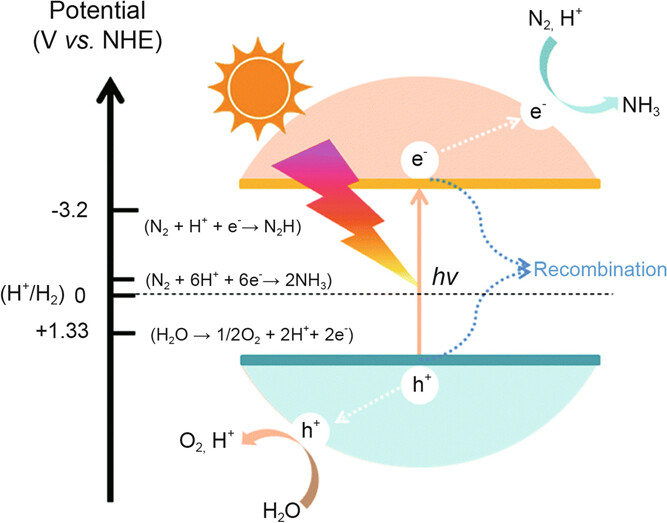
\includegraphics[width=0.6\textwidth]{figures/proposal_figures/Schematic_Sun.jpg}
\caption{Schematic illustration of the photocatalytic reaction process of a semiconductor. Image from Sun et al. \cite{Sun2023RecentReaction}.}
\label{fig:chen_photocata}
\end{figure}

% history of photocatalysis
In recent years, photocatalysis has emerged as a novel alternative for nitrogen fixation, utilizing abundant feedstocks of sunlight, water, and air. The concept of photochemical nitrogen transformations can be traced back to the early 20th century, when Indian soil scientist N.R. Dhar reported enhanced ammonia formation upon illuminating hydrocarbon-rich soils \cite{DHAR_1932}. Although these early observations were interpreted through now-disproven theories of radiation-induced reactivity \cite{lindemann1922discussion, Rao1932}, they laid important groundwork for the modern field of nitrogen photocatalysis. In 1977, Schrauzer and Guth demonstrated nitrogen fixation on UV-illuminated TiO$_2$ surfaces \cite{schrauzer1979nitrogen}. Since then, numerous efforts have been made to validate light-driven processes for ambient ammonia synthesis. However, despite decades of research, the reproducibility of photocatalytic nitrogen fixation and its underlying mechanisms remain subjects of ongoing scrutiny and debate \cite{Edwards1992, Davies1993, Davies_2007, hirakawa2017photocatalytic, Huang2023FormationIllumination, Huang2024BenchmarkingReaction}.

Following these early investigations, interest in photocatalytic nitrogen fixation has grown substantially, with efforts focusing on a broad range of photocatalyst materials \cite{Medford_2017, Hirakawa_2017, cao2019photocatalytic, hu2016effect, zhao2019tuning, jia2019site, cheng2019photocatalytic, Zhang2020NanostructuredFixation, comer2018role, Hao2020CatalyticProspects, Nazemi2019Plasmon-enhancedNanocages, Chang2020AuAmmonia}. Photocatalysis relies on semiconductors, typically deployed as particles or thin films in slurry-based systems or as photoelectrodes. Upon exposure to solar energy, these materials absorb photons and generate electron–hole pairs, which initiate redox reactions that drive nitrogen activation and reduction. Common photocatalyst candidates include metal oxides such as TiO$_2$, BiOBr, and Fe$_2$O$_3$, as well as graphitic carbon nitride (C$_3$N$_4$) \cite{Liang2020InsightDopant, hirakawa2017photocatalytic}. In oxide-based semiconductors, photon absorption with energy exceeding the band gap promotes electrons from the valence band (VB) to the conduction band (CB), leaving behind positively charged holes in the VB \cite{Sadeghfar2021ChapterMedia}. The electron–hole pairs generated during this process may recombine and release energy as heat, or they may migrate to the catalyst surface and participate in redox reactions \cite{Gaya2013HeterogeneousSolids}. The excited electrons in the conduction band can diffuse to surface active sites, where they reduce adsorbed nitrogen species. Meanwhile, the photo-induced holes in the valence band can also reach the surface and drive oxidation reactions. These holes possess strong oxidative potential, allowing them to directly oxidize adsorbates into reactive intermediates \cite{Lee2016RecentReview}. 

% limitations: reduce need for air separation
Similar to the Haber-Bosch process, current progress on photocatalytic nitrogen fixation relies heavily on pure nitrogen feedstock, which requires energy-intensive air separation. Liu et al. conducted a techno-economic analysis showing that the cost of nitrogen purification is one of the most sensitive variables in determining the levelized cost of ammonia (LCOA) for decentralized systems. For small-scale reactors (0.1–1 tN$_2$/day), membrane-based separations cost \$0.05–0.1 USD/kgN$_2$, significantly impacting overall economics. Eliminating air separation, by operating directly in air, could substantially reduce costs. For example, at a solar-to-ammonia efficiency of 10\%, the LCOA drops to as low as 30–120 USD/tNH$_3$ without air separation, compared to 110–200 USD/tNH$_3$ with it, a 60–270\% increase depending on the reactor architecture. The cost sensitivity to air separation is especially pronounced in low-capital, decentralized systems such as slurry-based photocatalytic reactors. Beyond cost, ambient operation introduces performance challenges: Hirakawa et al. found that the activity of rutile TiO$_2$ has been reported to decrease by 65\% under ambient air compared to purified N$_2$ environments \cite{Hirakawa_2017}. Under such conditions, oxygen can react with photogenerated electrons and holes to form reactive oxygen species, thereby lowering nitrogen conversion efficiency \cite{Ye2017Ni2PLight, Huang2020TowardLigands, comer2018role}. Therefore, eliminating the need for nitrogen purification is not only an economic imperative but also a technical one. Achieving this goal will require the development of photocatalysts that are selective and stable under aerobic conditions, capable of activating N$_2$ without being outcompeted or deactivated by O$_2$. The discovery of such air-compatible catalysts would be transformative for decentralized ammonia synthesis. This need directly motivates the work presented in this thesis in Chapter xx. 

% removing the air separation step is critical to enabling cost-effective, decentralized ammonia synthesis. Doing so will require the development of photocatalysts that are selective and stable under aerobic conditions that are capable of activating nitrogen without being poisoned or outcompeted by oxygen. Hence, discovering photocatalysts that are directly compatible with air or low-purity nitrogen is an important step towards enabling the photocatalytic NRR process under ambient conditions. 

% limitations: low performance
Despite extensive efforts to develop photocatalysts for the photocatalytic nitrogen reduction reaction (pNRR), current NH$_3$ yields remain far too low to support mass production \cite{Wei2022RecentBeyond}. Recent benchmarking studies have shown that many oxide- and carbon–nitride-based materials previously reported as active for pNRR exhibit negligible reaction rates upon rigorous validation \cite{Huang2024BenchmarkingReaction}. These low yields make experimental outcomes highly susceptible to contamination from adventitious NH$_3$ and nitrogen-containing impurities in the environment. This situation mirrors the issues with false positives in the electrocatalytic nitrogen reduction reaction studies; several catalysts once considered highly active were later shown to be inactive under more controlled experiments \cite{Andersen2019AMeasurements, Choi2022ReassessmentElectroreduction, Hao2022ReplyElectroreduction}. By testing with a custom-built stainless steel photoreactor, standardized cleaning protocols and carefully designed control experiments, Huang et al. show that three photocatalysts—Fe-BiOBr, g-C$_3$N$_4$/Fe$_2$O$_3$, and TiO$_2$ with oxygen-vacancy (OV-TiO$_2$) exhibited no measurable activity for pNRR under illumination. Therefore, more rigorous control experiments are necessary to ensure the reproducibility and reliability of photocatalyst activity.


% \section{Innovative Approach to Sustainable Fertilizer Production}
\section{Avoiding Nitrogen Fixation with a Circular Nitrogen Economy}
Although much of the research on sustainable ammonia production has focused on improving or replacing the Haber–Bosch process with greener alternatives, such as photocatalysis and electrocatalysis, an intriguing alternative strategy is to avoid nitrogen fixation altogether. Instead of converting inert atmospheric N$_2$ into reactive nitrogen species, a circular nitrogen economy seeks to recover and reuse existing reactive nitrogen from waste streams \cite{Botte2024InnovativeRecovery, ChipocoHaro2024ElectrocatalystsConversion, Ferreira-Garcia2025ElectrochemicalEconomy, Okoye2025NitrateProduction, Coyle2025NovelCarbon, AlvarezPugliese2024EfficientElectrodes, Abbasi2024FundamentalsCompound, botte2023methods}. This paradigm shift reframes the challenge from increasing global fixed nitrogen supply to managing and recirculating what has already been introduced into the biosphere.

\subsection{Drivers for nutrient recovery}  
Nutrient pollution from agricultural sources, mostly from crop fertilization and manure from livestock operations, poses a growing ecological concern worldwide through water and air pollution \cite{DelRossi2023TheAgriculture}. In the US, agriculture is the most significant contributor to nitrogen pollution, accounting for more than 50\% of nitrate, ammonia, and nitrous oxide emissions \cite{Ribaudo2011NitrogenPolicy}. Excess fertilizer-derived nitrate (NO$_3^-$) and nitrite (NO$_2^-$) leached from agricultural soils are the main contributors to water pollution, leading to eutrophication, hypoxia, loss of biodiversity and harmful algae growth that threaten sensitive ecosystems such as coral reefs \cite{Jung2021MaterialProduction, Bijay-Singh2021FertilizersProblem}. In industrialized regions of North America and Europe, surface and groundwater nitrate contamination has been a recognized problem since the 1970s, resulting from decades of intensive fertilizer use \cite{Mateo-Sagasta2018MoreAgriculture}.

In addition to inorganic nitrogen, growing levels of organic nitrogenous compounds, including urea, amino acids, pharmaceuticals, pesticides, and dyes, pose emerging environmental and health challenges \cite{Zheng2021DissolvedImpacts, Chen2011OccurrenceNitrogen}. These compounds originate from both agricultural runoff and internal processes within wastewater treatment plants, where up to 50\% of dissolved organic nitrogen can be generated during biological treatment \cite{Zheng2021DissolvedImpacts}. With growing global populations and expanding access to wastewater infrastructure, the prevalence of organic nitrogen waste is projected to rise \cite{Seiple2017MunicipalStates}. Once released into aquatic environments, these compounds not only intensify eutrophication but can also form hazardous byproducts during treatment, posing long-term public health risks \cite{Sillanpaa2018RemovalReview}.

\subsection{Electrochemical Fertilizer Recovery from Sludge Waste}
In addition to removing harmful nitrogen species from wastewater, nutrient recovery technologies can also enable the production of fertilizers. One promising approach involves electrochemically treating waste activated sludge (EWAS) to create sustainable fertilizers \cite{Coyle2025NovelCarbon, botte2023methods}. This process supports a circular nitrogen economy by both mitigating waste and recovering nutrients from waste streams such as animal waste and runoff \cite{Rodriguez-Espinosa2023NitrogenEconomy}. The electrolysis process reduces sludge volume and pathogen content and increases the concentration of bioavailable nutrients \cite{JafariElectrochemicalProduction, JafariElectrochemicalProduction}.

According to Coyle et al., the EWAS-treated soils released less total nitrogen into the solution compared to commercial fertilizers, mainly due to organoclay complexation and reduced solubility of nitrogen species \cite{Coyle2025NovelCarbon, Marschner2008HowSoils}. At the same time, EWAS showed enhanced carbon solubility, attributed to the structural deformation of organic matter caused by the alkaline electrolysis process \cite{Sparks2003ChemistryMatter, Chen1976ScanningComplexes}. These characteristics indicate that EWAS can help reduce nutrient runoff, enhance soil health, and facilitate localized fertilizer production, thus contributing to broader sustainability goals.

Despite these benefits, significant challenges remain in implementing EWAS at scale. The electrochemical process must contend with variable feedstock composition, high solids content, and corrosion of electrode materials during operation \cite{Abbasi2024FundamentalsCompound, Ferreira-Garcia2025ElectrochemicalEconomy, JafariElectrochemicalProduction}. Most electrocatalysts are not optimized for the harsh and heterogeneous environment of sludge, which can include organic acids, microbial byproducts, and corrosion-inducing ligands \cite{Barragan2021LeachingOptimization, lekfeldt2017heavy, das2021studies, iqbal2015leaching}. These harsh conditions contribute to catalyst degradation and reduce the operational lifetime of electrochemical reactors. Understanding how and why this degradation occurs under realistic nutrient recovery conditions is therefore critical. The final chapter of this thesis addresses this need by investigating catalyst stability during EWAS treatment to inform future materials design and improve the longevity and efficiency of electrochemical nutrient recovery systems. 



\section{Overview of Thesis Chapters}

This thesis includes detailed computational studies related to sustainable ammonia synthesis: photocatalytic nitrogen fixation, photo(electro)catalytic ammonia synthesis from air, and electrocatalytic conversion of waste sludge to ammonia. A detailed summary of each technical chapter is provided below. 

\subsection{Carbon Radical-Assisted Nitrogen Activation on Titania}

The discovery that carbon radicals can promote the activation of dinitrogen has reshaped the photocatalysis community's understanding of titania-based nitrogen reduction \cite{comer2018role, Huang2023FormationIllumination}. Titanium dioxide (TiO$_2$), long regarded as the archetypal photocatalyst, was traditionally evaluated under the assumption that nitrogen activation proceeds via direct electron transfer at oxygen vacancies or surface-bound hydroxyl groups. However, electron paramagnetic resonance (EPR) and infrared (IR) spectroscopy studies reveal the formation of diazo and nitrogen-centered radicals when methanol—a common hole scavenger—is used under UV illumination. These intermediates arise from surface-bound carbon radicals, such as CH$_3^\cdot$ and CH$_2$OH$^\cdot$, reacting with N$_2$ to form CH$_x$N$_2^\cdot$ species.

Density functional theory (DFT) simulations indicate that carbon-derived intermediates, such as those formed from methanol, significantly reduce the thermodynamic barriers for dinitrogen activation, thereby providing a viable pathway to ammonia formation. Although demonstrated on titania, this mechanism likely extends to other semiconductors capable of oxidizing organic compounds. These insights challenge the long-standing assumption of N$_2$ inertness in photocatalysis, suggesting that hole scavengers may play an active, catalytic role in nitrogen conversion processes.

\subsection{Screening Metal Compound Active Sites for Selective N$_2$ Adsorption}

To advance nitrogen fixation technologies beyond model TiO$_2$ systems, a high-throughput computational screening framework was developed to identify materials with strong and selective adsorption of N$_2$ over O$_2$. The rationale stems from a critical barrier to ambient nitrogen fixation: the presence of oxygen in air. Industrial processes rely on cryogenic distillation to obtain pure N$_2$, but this adds significant energy and capital costs. Thus, photocatalysts that can selectively adsorb nitrogen while resisting oxygen poisoning are needed.

Using a two-stage density functional theory (DFT) workflow, over 2500 active sites derived from 516 metal oxide, oxyboride, and oxyphosphide bulk structures were evaluated. In the first screening stage, the adsorption energies of N$_2$ and O$_2$ were computed on fixed slabs, and promising candidates exhibiting favorable selectivity were identified. A second round of calculations allowed surface relaxations, revealing that metastable polymorphs of TiO$_2$ and a vanadium borate (VBO$_4$) surface retained strong and selective N$_2$ adsorption. Detailed pathway analysis using BEEF-vdW and HSE06 functionals confirmed that these active sites not only adsorb N$_2$ selectively but also exhibit thermodynamic barriers comparable with the canonical rutile TiO$_2$ (110) surface.

This work demonstrates that adsorption selectivity is a valuable descriptor for identifying photocatalysts that operate effectively in ambient air. Under realistic conditions, N$_2$ must compete with O$_2$, H$_2$O, CO$_2$, and other airborne molecules that may occupy active sites or form interfering surface intermediates. By focusing on materials that selectively bind N$_2$ while limiting the adsorption of more reactive species, this screening framework addresses a major challenge in nitrogen fixation under ambient conditions. The results also emphasize the potential of metastable materials as sources of uniquely selective and active surface sites.

\subsection{Stability of Electrode Materials for Electrochemical Nutrient Recovery}

While photocatalysis enables decentralized ammonia synthesis, the electrolysis of waste-activated sludge (EWAS) provides an alternative strategy for nitrogen recovery from wastewater streams. However, designing sustainable catalyst materials remains a key challenge, as nitrogen-containing ligands and pulsing reductive–oxidative potentials can cause significant corrosion of conventional electrode materials.

This section outlines a computational strategy to assess the electrochemical stability of metal and alloy catalysts in the presence of nitrogen-containing ligands. By extending the classical Pourbaix diagram formalism to include ligand effects from ammonia, glycine, and cyanide, the framework captures how waste-derived species influence material dissolution and passivation behavior. Results reveal that while noble metals like Ni and Au are highly active, they form soluble glycine complexes under EWAS conditions. In contrast, Ti and Ti-based alloys exhibit robust stability across a wide pH potential range due to the formation of passive oxide layers, making them ideal candidates for long-term use.

Complementing bulk thermodynamic insights, Monte Carlo simulations and machine-learned interatomic potentials were used to explore surface composition and adsorbate coverage. These studies uncovered that surface passivation, particularly by oxygenated species or ammonia, can modulate corrosion resistance and should be included as a design criterion alongside catalytic activity.

\section{Outlook}

The studies presented in this thesis combine mechanistic insights, high-throughput screening, and stability analysis to address the complex challenges of nitrogen conversion. From the unexpected role of carbon radicals in N$_2$ activation to the identification of selective photocatalysts and finally to the analysis of catalyst stability in EWAS, each component contributes to a more holistic understanding of the sustainable chemistry of nitrogen.

% The convergence of spectroscopy, theory, and data-driven materials discovery offers an exciting pathway toward rational catalyst design. Future work should extend this approach to multicomponent systems, incorporate kinetic effects, and integrate experimental validation to accelerate the deployment of sustainable nitrogen technologies.

